\chapter{Review of computational drug repositioning approaches}

\textbf{Key points}
\begin{itemize}
  \item Drug repositioning is the discovery of new indications for approved or failed drugs.
  \item Repositioning opportunities exist because drugs perturb multiple biological entities (on and off-targets) themselves involved in multiple biological processes. As the drug discovery pipelines are focused on one disease of interest, a therapeutic application for a drug to other areas can be missed.
  \item A variety of predictive computational approaches have been developed to identify drug repositioning opportunities, each based around a biological concept of interest.
  \item For my thesis, I decided to investigate drug repositioning using the concept of mode of action. This notion is of interest as it can represent the various biological functions a drug can play in an organism and help to identify new therapeutic applications.
\end{itemize}

\textbf{Author’s comment}

This chapter is a review of the computational methods developed in the last decade, presenting their relative strengths and weaknesses. This state-of-the-art analysis helped me to define the rationale for my thesis.

Living organisms, just as machines, are subject to dysfunction. Sometimes an internal abnormality can impair the correct functioning or sometimes external forces, such as the interaction with the environment, can damage a body. If not fixed, malfunctions accumulate and will eventually result in the death of the entity, namely the cessation of all functions. Since prehistoric times \citep{prehistoricwiki}, humans have been interested in preventing and handling dysfunctions, in order to extend the lifespan of objects or to improve the quality of their own existence. When the aim is to fix living bodies, this practice goes by the name of medicine, or the art of preventing, diagnosing and treating diseases.

Alleviating an impairment is a daunting task, from both a biological and legal perspective. In this regard, doctors can rely on a number of tools, engineered throughout the years. Among the most commonly used ones such as medical devices, are the active small molecules, the drugs. Drugs are of primary interest, as they can impact the treatment of complex processes with molecular roots, such as cancer or pain for instance, in a relatively controllable and safe manner. However, in order to be usable in clinics, a candidate drug has first to go through a development phase which takes nowadays at least a dozen years and can cost up to a billion dollars \citep{dimasi2001new}. This process involves a myriad of different people, from biologists to law attorneys.

As my interests revolve primarily around pharmacology and computer sciences, I decided to focus my efforts on the molecular side of the problem. More precisely, I decided to systematically characterise and understand the multiple roles any drug can play in the human body, using computational means. My work will be extensively described throughout this manuscript and finds an application in a topic named drug repositioning, which is the object of this chapter.

\section{Relevance of drug repositioning}

Drug repositioning (also referred as drug repurposing, re-profiling, therapeutic switching and drug re-tasking) is the identification of new therapeutic indications for known drugs. These drugs can either be approved and marketed compounds used daily in a clinical setting, or they can be drugs that have been "shelved", namely molecules that did not succeed in clinical trials or for which projects have been discontinued for various reasons. In one sentence, drug repositioning can be defined as \emph{renewing failed drugs and expanding successful ones} \citep{barratt2012drug}.

One motivation behind drug repositioning is the possibility to further market and extend the application line or patent life of a drug, therefore increasing the revenue stream generated from it. Another aim is the treatment of rare or neglected diseases; usually such conditions are difficult to address for financial reasons, yet there might exist some safe and active molecules already developed for other indications, deemed suitable for this scenario \citep{men20101}. I refer the reader to some recent excellent reviews (//cite reviews) in order to fully appreciate the economical market behind this approach, as well as legal challenges coming along. I limited myself, in the context of this work, to exploring the subject from an academic perspective: Characterising the various roles approved drugs can play using computational means, without necessarily seeking business opportunities.

\subsection{Opportunities for finding new indications}
\label{sec:opp}

Many drugs have been successfully repositioned in the past; classical examples such as sildenafil (Viagra) and thalidomide will be presented in the coming sections. But first, the scientific legitimacy of the idea behind drug repurposing should be discussed: How is it possible for a drug to play multiple roles? What is the molecular rationale? Why does the drug discovery process not automatically identify such opportunities?

In order to be able to answer these questions, I will briefly present the traditional drug development pipeline, which produced most of the recent therapeutic chemicals \citep{swinney2011were}.

The fundamental idea behind the discovery of a new medicine has not evolved much since prehistoric times \citep{prehistoricwiki}; it still consists mostly of a trial and error process, hence the term "discovery". The operation starts by picking a disease of interest, selected in terms of market size or clinical needs. Then a large collection of chemicals is experimentally tried to see if any relevant effect in regards to the chosen condition can be produced. This procedure is called screening. There exist mostly two types of screening: target-based and phenotypic. The former optimises the selection of the chemicals on the ability to bind a biological entity (usually a protein), called the target and that is relevant for the pathological process studied. The more specifically the chemical interacts with the active site of the target, the cleaner the action of the chemical will be (key-lock model - see Figure \ref{fig1-1}).

\begin{figure}[ht]
    \centering
    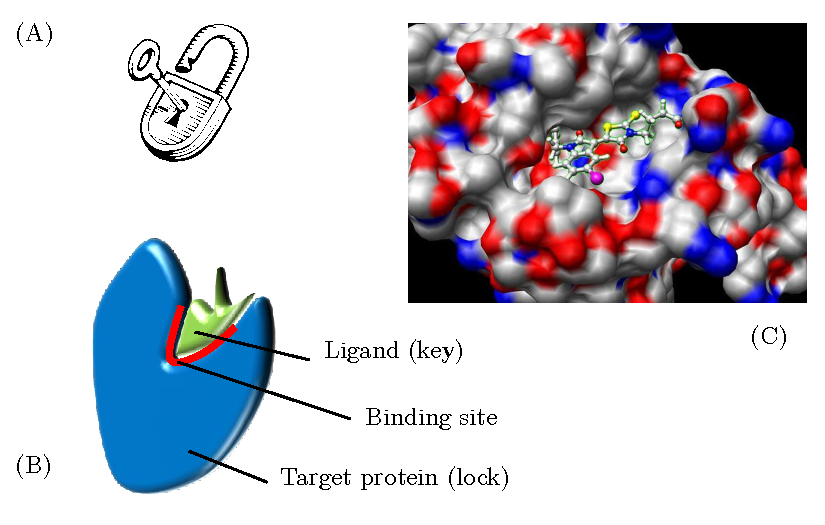
\includegraphics{fig1-1}
    \caption{Key-lock model. (A) Illustration of the analogy. (B) Schematic representation of the interaction between a ligand and a protein (receptor, enzyme, transporter, etc). One aim of drug discovery is to find alternative molecules (i.e. drugs) capable of either mimicking the action of the natural ligand or reversing it. In theory, the more specific the molecule is to the binding site, the more accurate the pharmacological response will be. (C) Computer generated representation of the interaction between a ligand and a protein. (Source http://en.wikipedia.org/wiki/File:Docking.jpg)}
    \label{fig1-1}
\end{figure}

On the other hand, a phenotypic screen does not make any assumptions about the underlying pathological mechanism and proteins involved. A cell line or model organism representative of the disease is directly used to read the results of the screening. Both methods help to efficiently discover active chemicals, whose structures are then further optimised for efficacy (so called \emph{lead optimisation}). Now drug repurposing opportunities can be derived from three key observations \citep{barratt2012drug} about the traditional workflow presented above and summarised in Figure \ref{fig1-2}.

\begin{figure}[ht]
    \centering
    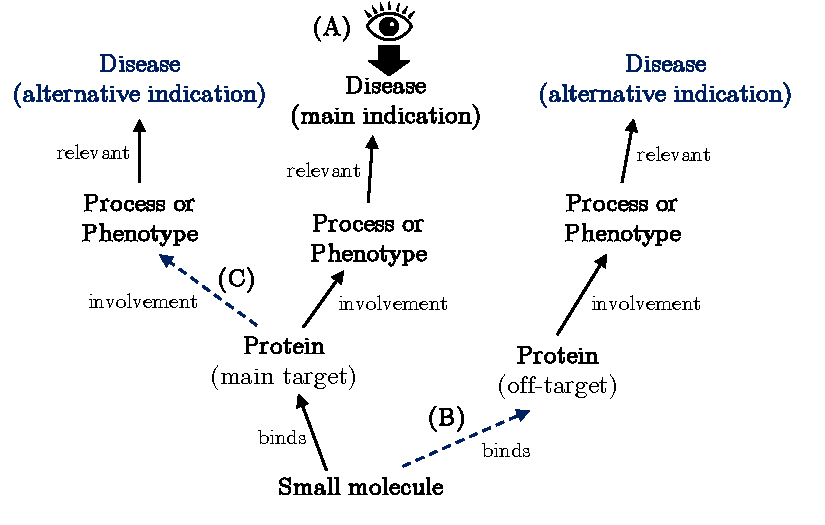
\includegraphics{fig1-2}
    \caption{Drug discovery process and opportunities for drug repositioning (in blue; logical connection at the origin of the opportunity are dashed). (A) Traditional drug discovery workflow: From biological evidences showing the involvement of a protein in a process relevant to a particular disease of interest, a series of chemicals are screened for bioactivity. Potent and safe molecules will become drugs indicated for the disease. Paul Ehrlich postulated that chemicals should be as specific as possible against the target (organism or protein), in order to increase the control over the pharmacology. The concept of "magic bullet" describes such an ideal therapeutic compound. (B) Repositioning hypothesis: Often, a small molecule binds to other proteins (so called off-targets), themselves potentially involved in other pathologies. (C) Repositioning hypothesis: The main protein target can be involved in a series of alternative biological processes and relevant for another disease.}
    \label{fig1-2}
\end{figure}

The first observation appreciates the limits of the key-lock model and the "magic bullet" concept \citep{ehrlichwiki}. In practice, it is extremely challenging to design a molecule that will interact with a single protein only \citep{paolini2006global} \citep{li2010pubchem}. Most of the drugs will bind to multiple proteins in an organism and can therefore produce a variety of unwanted effects (concerns between 35 to 62\% of the chemicals - sometimes described as "drug promiscuity"). This characteristic is well-known and referred to as off-target effect or polypharmacology. Identifying the off-target proteins interacting with known drugs can provide repurposing opportunities.

The second observation values evidence that molecular targets are themselves involved in multiple biological processes and capable of performing multiple functions. Historically speaking, one protein target was assumed to be responsible for one biological role. Hitting the right protein, such as a receptor or an enzyme known to be directly involved in the disease was a straightforward way to generate relevant phenotypic outcomes, as illustrated in Figure \ref{fig1-2}. However, this approach overlooks the fact that proteins function in the context of signalling pathways and networks (//cite network biology paper), the perturbations experienced by one node cascading on to its neighbours due to molecular dynamism. Therefore understanding and appreciating the involvement of the protein target in the biological system can help to identify a new role for a drug.

The last observation derives from the very strategy used by drug discovery programs. As a disease or condition is the starting point of the screening, identified chemicals are by definition optimised in this regard. Compounds will be tested during the expensive clinical trials for the main indication mostly and obviously not for all possible diseases. It is therefore possible for a compound to be used for different purposes, yet not be identified as such. Related to this, new usages can be discovered during clinical practice, and the prescription of the drug can evolve accordingly even if the alternative indication is not legally approved. This practice is known as off-label prescription \citep{offlabelwiki} and demonstrates the potential of a drug to address various indications.

To conclude, these three observations alone justify the potential existence of repositioning opportunities, especially for the drugs discovered via the target-based or phenotypic screening. Meaningful repurposing options appear to be strongly dependent on the available biomedical knowledge, as well as our understanding of the molecular system.

\subsection{Drug repositioning faces legal and scientific challenges}

In theory, it is possible for a chemical to be active for multiple therapeutic indications. Yet in practice, several obstacles can impair the development of a potential new usage.

The first factor to handle is serendipity. Biology is complex and capricious, exemplified by diseases such as cancers or dementias (//cite something). A drug rarely keeps its original indication \citep{barratt2012drug}; it gets reoriented throughout the years when more data becomes available and its in vivo pharmacology better understood. Famous repurposing and discovery stories were mostly due to chance and unexpected results (e.g. the Viagra, as will be discussed), therefore it can be difficult to forecast any relevant opportunities.

Other challenges come from the corporate and legal aspect around drug discovery. Indeed, in order to be commercially valid, a molecule needs much more than just to exhibit powerful pharmacological features. If the intellectual properties around the molecule are expired or close to be, there might be no incentive to continue the research on an alternative indication, as no profit would derive from it. Re-indicating a drug is also not part of the standard regulatory procedures, therefore administrative problems can happen, delaying or preventing the new usage of the compound. Moreover, some unnecessary safety concerns could appear when the drug is tested for the new indication. Indeed, the repositioning would potentially target a different group of patients, with different physiological conditions, and it is not to be excluded that an unforeseen adverse event could happen during the trials over the new population, hence compromising the original indication.

The dosage at which the drug is administered could also be a potential obstacle; the molecule still needs to preserve a good efficacy and show some activity at low concentration. Depending on the anatomical part of the body targeted, the formulation should also be reconsidered for efficacy. These factors can alter the pharmacokinetic profile of the drug and compromise the safety of the patient.

To conclude, the molecular opportunities for drug repositioning are contrasted by practical challenges. Even if a compound is found to be active and safe for a new indication, additional factors, in particular legal issues and intellectual property, have to be considered in order to successfully bring the molecule to the market.

\section{Drug repositioning and indication discovery: Success stories}

I discussed briefly in the previous section the theoretical legitimacy of drug repositioning and its potential limitations. I will now present three success stories, exemplifying the theory and showing evidence that repositioning can happen in practice. These case-scenarios are of particular interest as they each illustrate a different reason behind the repurposing. Understanding the logic backing the findings is paramount in order to build successful predictive methods later on.

\subsection{Sildenafil: Repositioning from clinical side-effects}

The National Health Service (NHS) defines angina as a chest pain that occurs when the blood supply to the muscles of the heart is restricted. It usually happens because the arteries supplying the heart become hardened and narrowed \citep{anginanhs}. Sildenafil (see structure in Figure \ref{fig1-3}) was originally developed for this condition in the late 1980s. The working hypothesis was that an inhibition of the activity of the phosphodiesterase-5 (PDE5), an enzyme controlling the relaxation of the coronary arteries, should increase the blood flow and release the symptoms in the patient. Unfortunately, during the clinical trials, the drug lacked efficacy in regard to angina and development was discontinued, until patients shily started to report an unusual side-effect: prolonged erections (personal discussion with molecule's investigator). Pfizer's scientists therefore decided to investigate the drug for this indication and a worldwide study of 3700 men confirmed the effectiveness of the molecule \citep{nytimes}. As the pharmacokinetic profile was suitable, the drug was repurposed towards erectile dysfunction accordingly. Viagra became a blockbuster drug, with annual sales higher than 1.5 billion dollars \citep{renaud2002erectile} during the first years of its release. The molecule was first-in-class for this indication and impacted the social life of millions of humans \citep{renaud2002erectile}. The story does not end here; the drug is currently used for pulmonary arterial hypertension too, after demonstrating a successful improvement in patients during clinical trials \citep{ghofrani2006sildenafil}.

\begin{figure}[ht]
    \centering
    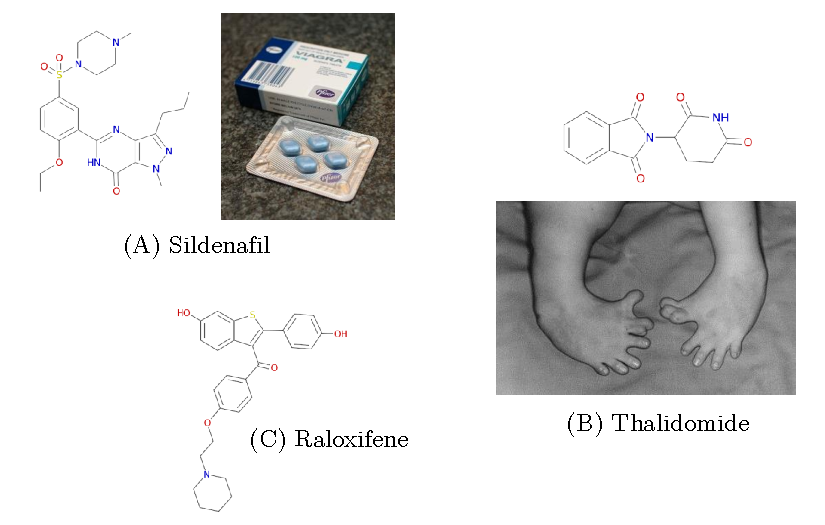
\includegraphics{fig1-3}
    \caption{Examples of drug successfully repurposed. (A) Sildenafil molecular structure and picture of tablets used for administration. (B) Thalidomide molecular structure. The teratogenic effect of the drug is illustrated on the picture. (C) Molecular structure of the raloxifene. Illustration are from Wikipedia, chemical structures from the ChEMBL database.}
    \label{fig1-3}
\end{figure}

What can be learned from this story? Firstly, the repositioning opportunities came from secondary functions of the enzyme targeted. PDE5 was known to be involved in the erection process \citep{krall1988characterization}, therefore the opportunity could have been logically identified rather than being discovered by pure chance. In this regard, characterising the systematic function of protein targets can therefore lead to repositioning hypotheses. Secondly, it was necessary to wait for clinical trials in order to observe the true behaviour of the drug. This observation stresses the known difficulty of moving from cell-based assays into the human body: physiology is complex and the expected outcomes are not necessarily met in practice. Lastly, the more is known about the compound’s pharmacology, the more roles the molecule can play, as shown with the indication for the pulmonary arterial hypertension, which appeared years later. An understanding of the internal logic of biological organisms should therefore help to predict such cases.

\subsection{Thalidomide: Repositioning a hazardous drug}

The story of thalidomide illustrates how a drug can surprisingly come back from being a hazardous drug retracted from the market into a novel and unique therapeutic agent. The chemical started its life in 1957 in Europe, as a sedative, sleep-inducing agent, structurally close to barbiturates (see structure on Figure \ref{fig1-3}). Because of these pharmacological properties, thalidomide was marketed to treat morning sickness in pregnant women. The drug was assumed to be safe, based on an in vivo studies in rodents \citep{stephens2009dark}. Tragically, this was not the case for humans; the drug caused severe skeletal birth defects in children born from women taking the drug. Over 15’000 newborns were affected, suffering from anatomical malformations (see Figure \ref{fig1-3}). Because of this disastrous side-effect, the molecule was quickly withdrawn and triggered important reforms in the drug regulatory system \citep{stephens2009dark}. The story could have ended here, if it were not for an incidental discovery by Jacob Sheskin. The practitioner was trying to treat patients affected by erythema nodosum leprosum, a particularly painful inflammatory condition characterised by red nodules under the skin. An evening of 1964, an affected patient could not sleep as the pain was so intense. Sheskin decided to ultimately use some thalidomide, as the compound was known for its potent sleep-inductive properties and was available in this hospital. The drug worked and the patient was well rested in the morning. And as a general surprise, all pain and soreness disappeared overnight too. Intrigued by the idiosyncratic effect of the drug, Sheskin further studied the action of thalidomide in clinical trials \citep{barratt2012drug} and successfully showed that the drug can indeed treat erythema nodosum leprosum in two weeks' time in most subjects. Thalidomide found a new life and became the first and only drug approved for this indication. Just as for the sildenafil molecule, the potential of the chemical is still being unveiled: At the time of writing, thalidomide sales are reaching over 200 million dollars per year, mostly deriving from yet another off-label use for multiple myeloma, among other indications (//cite nature review 2004). The thalidomide story teaches us that a drug can be harmful in one patient population (pregnant women) and highly beneficial in another. Correctly identifying the molecular processes affected can help to predict adverse effects and reorient the drug accordingly. The root cause of the discovery is here again serendipity, yet a better understanding of the proteins interacting with the molecule could have been helpful to predict the opportunity \citep{sampaio1991thalidomide}.

\subsection{Raloxifene: Expanding the application line}

The last case discussed is less striking and unexpected than the two previous ones. Raloxifene (structure on Figure \ref{fig1-3}) is a selective estrogen receptor modulator (often abbreviated as SERM) marketed as Evista by Eli Lilly. Similarly to other estrogen modulators, such as tamoxifen, the original indication during preclinical developments was breast cancer (//cite nature review). Despite early studies showing the positive effect of antiestrogens on osteoporosis in rats in 1987 \citep{jordan1987effects}, raloxifene's potential for this usage was not experimentally confirmed until 1994 \citep{black1994raloxifene}. Eventually, the molecule successfully passed clinical trials in 1999, with osteoporosis as a unique indication. However, the polypharmacology of the drug, particularly its action against breast cancer, was still under investigation. Finally, in 2007, the FDA approved raloxifene as a preventive agent for breast cancer in postmenopausal women \citep{fdaraloxifen}, therefore extending the line of application of the drug back to its originally thought indication. In summary, raloxifene started its life as a breast cancer agent, was repositioned against osteoporosis, likely for strategic and commercial reasons, and eventually got approved for its breast cancer preventive properties. This drug is an example of smart and continuous development, expanding from one indication to another. The fundamental reasons behind the repositioning are grounded on early-stage experimental evidence and not due to a surprising effect appearing in clinical trials. The drug's polypharmacology was known and the indication of the molecule derived accordingly. Raloxifene is a good example of "educated repositioning" or indication discovery. The available information can help to appreciate and understand what the chemical might do from empirical evidence.

\section{Computational approaches towards drug repositioning}
\label{approaches}

The theory and the clinical cases presented the reality of drug repositioning. I briefly commented on the fundamental reasons enabling new usages and stressed the importance of serendipity in this process. Now the fantasy of many scientists working in the drug discovery domain is to be able to formally predict such repositioning scenarios and unveiling new pharmacology in an automated fashion. In order to reach this distant goal or at least get closer to it, several computational approaches have been developed throughout the years. This section summarises the previous work done on the topic and motivates the novel way I explored, based on a formal representation of the Mode of Action (MoA). I chose to classify the different computational approaches based on the biomedical concepts used as the centre of the methodology. Some recent reviews (//cite nature review) \citep{dudley2011exploiting} \citep{hurle2013computational} of the field can also provide complementary information to the interested reader, as well as a different perspective and logical structure of the topic.

Abstracted to the extreme, the goal of a repositioning initiative is to establish a link between a drug and a disease. This edge represents the indication or a prescription possibility for the molecule. In order to computationally forward new indication hypotheses, it is possible to use the biomedical concepts depicted on Figure \ref{fig1-4} as proxy. Usually, a similarity value is derived from the property studied (e.g. chemical structure or gene expression level), which serves as a descriptor to rank the information and predict the new indication, materialised by a new link between a drug and a disease or a molecular target. Approaches can be roughly divided into groups, named after the central property of the analysis. Some alternative methods rely on a combination of concepts and are presented at the end of this section.

\begin{figure}[ht]
    \centering
    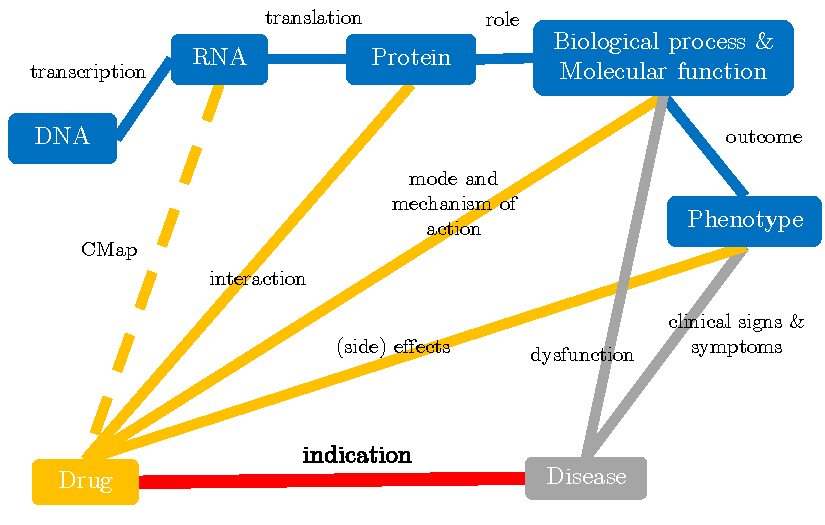
\includegraphics{fig1-4}
    \caption{Conceptual map of the relationship between the different biomedical concepts. Relation related to the drug and its action are in orange, diseases in grey and biological concepts are in blue. Computational drug repositioning methods are based on either one or a series of such concepts in order to forward new indications for a drug, ultimate goal (red edge).}
    \label{fig1-4}
\end{figure}

\subsection{Chemical structure-based approaches}

Traditionally speaking, orally active drugs are mostly small lipophilic molecules \citep{lipinski1997experimental}. It therefore intuitively makes sense to directly look at the chemical structure to compare the similarity among drugs: Similar structures are deemed to lead to similar biological outcomes. This rule of thumb goes by the name of "similar property principle" \citep{johnson1990concepts} and is at the core of any quantitative structure-activity relationship (QSAR) study. A variety of methodologies exist to calculate the structural similarity between two chemicals, such as fingerprints or clustering algorithms \citep{eckert2007molecular}. These methods can be used to perform ligand-based virtual screenings: from a set of known active ligands, trying to find in a database of interest the structurally related molecules, supposedly bioactive too.

In the context of drug repositioning, one can search only among approved compounds for instance. This approach was successfully used by \cite{noeske2006predicting} implementing an unsupervised machine learning algorithm (self-organising map) in order to cluster chemicals based on their structure. Molecular scaffolds were represented as vectors and used as input for the clustering step. The authors identified cross-activities for the metabotropic glutamate receptor antagonists, on other protein targets such as the dopamine D2, histamine H1 and muscarinic acetylcholine receptors. The off-target predictions were experimentally validated in vitro and shown to be active, yet not necessarily pharmacologically relevant due to weak binding. The new knowledge on off-target binding from this study can lead the way to potential new usage for the drugs, by further modifying and optimising the molecular structure for instance.

Another interesting approach related to structural similarity for off-target identification comes from the work done by \citep{keiser2009predicting}. For this project, known ligands were grouped based on their known target binding partners and chemical features. The method is called "similarity ensemble approach" and "calculates whether a molecule will bind to a target based on the chemical features it shares with those of known ligands, using a statistical model to control for random similarity" (\cite{lounkine2012large} - adaptation of BLAST for chemical structures). In the case of drug repositioning, the molecules tested were only approved drugs. The results revealed a series of off-target cases from the similarity analysis. A retrospective investigation showed the validity of the approach; then some predicted off-target bindings were experimentally validated, providing insightful clues about the pharmacological mechanism of some drugs. In some cases, such as for fabahistin, the off-target affinity (5-HT5A) was even better than for the known canonical receptor (H1), opening doors for meaningful alternative indications (see Figure \ref{fig1-5}).

\begin{figure}[ht]
    \centering
    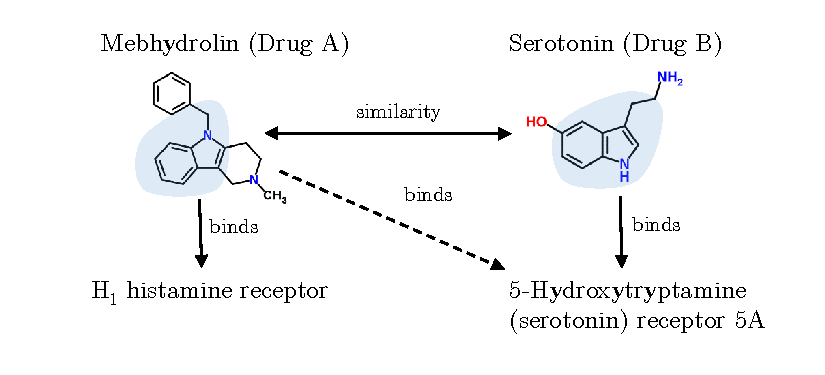
\includegraphics{fig1-5}
    \caption{Drug repositioning using the chemical structure. Compounds with similar structures have similar biological activities (similarity principle). Molecule (A) shares some similarity with molecule (B), indicated by the blue areas. This observation leads to the conclusion that molecule (A) could be active on the canonical target of molecule (B), and indicated accordingly. See \cite{keiser2009predicting} for full details on example. Structures obtained from the ChemSpider database.}
    \label{fig1-5}
\end{figure}

Chemical-based approaches are intuitive and build on the accepted "similar property principle" (see Figure \ref{fig1-5} for summary). However in practice, small changes made to a molecular structure can lead to drastically different biological outcomes. Moreover, the predictions made by the various methodologies have little overlap between them, stressing the difficulty to select the adequate one for the right scenario \citep{eckert2007molecular}. Some compounds also undergo chemical modifications by the cell before being pharmacologically active, therefore the structure as recorded in databases can compromise the value of a predictive statistical model. Finally, by using potent and optimised molecules as starting point to infer new ligands or to train a model, there is a high risk that the predictions will manifest weak experimental pharmacology for the new indication. Indeed, such inferred compounds are not "dissimilar" enough to have an unexpected binding conformation with the protein and any differences in structure against the endogenous ligand will only reduce potency.

\subsection{Gene expression and functional genomics-based approaches}
\label{expression}

Living systems can be understood by looking at the behavior of their gene expression in a particular setting. Depending on the state of the system, certain genes are going to be over or under expressed, identifiable from the relative number of their messenger RNA (mRNA) molecules transcribed. Differentially expressed genes can serve as a proxy to characterise a molecular effect, so called the gene expression signature. This type of experiment is usually performed on a microarray, containing probes for the genes of interest (see Figure \ref{fig1-6}A). The approach provides a straightforward read of the condition studied and has been successfully used to find new indications for marketed drugs. In particular, the Connectivity Map \citep{lamb2006connectivity}, was behind most recent repositioning stories (see Figure \ref{fig1-6} for summary of the method).

\begin{figure}[ht]
    \centering
    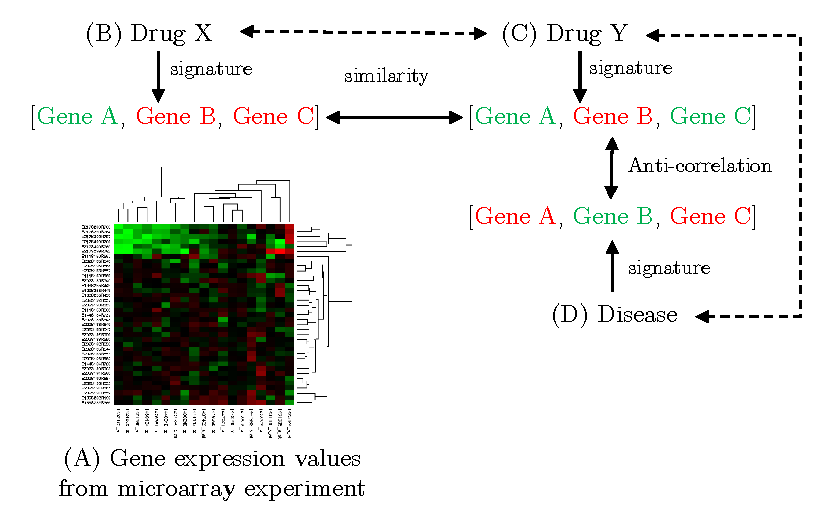
\includegraphics{fig1-6}
    \caption{Drug repositioning using gene expression. (A) Example of result obtained from a gene expression experiment. Some of the probed genes are up-regulated (green), some of them down-regulated (red). (B) and (C) The gene expression data from the Connectivity Map provides a signature which can relate drugs on their functional aspect. For instance drug X and Y are considered similar because they share a significant amount of genes up and down related. (D) An analog reasoning can be made with the relation drug-disease: Disease signature can be treated by drugs with an anti-correlating signature.}
    \label{fig1-6}
\end{figure}


The idea behind the CMap states that the action of a drug can be captured and compared by looking at the gene expression profile resulting from its administration onto a biological system. In this regard, the initiative recorded the molecular signatures of 164 FDA-approved molecules over 5 different cancer cell lines. The data is freely available and can help to perform various type analyses, for instance related to the understanding of the molecular mechanism of a drug.

Closer to my concerns, \citep{iorio2010discovery} used the resource for drug repositioning, by comparing small molecules on the basis of their CMap gene expression signatures: Compounds with similar signatures were assumed to be functionally related, as they perturb the cell in a similar fashion. On this basis, the researchers identified communities of drugs sharing known protein targets and mechanism of actions. Interestingly, inside these hubs, most of the drugs were also sharing the same or similar therapeutic indications; yet outliers were present. Such cases were interpreted as repositioning opportunities, as these compounds appeared similar on the signature level (same gene expression profile), yet were clinically used for different purposes. Based on these considerations, the authors discovered that fasudil, a potent vasodilator, can also be used as an enhancer of cellular autophagy. The prediction was experimentally verified on standard cell assays. The novelty of the methodology lies in the way variable gene expression data from different cell lineages was integrated in order to derive meaningful metrics.

Messenger RNA expression can reflect the activity of a drug, but it can also be used to characterise disease states. Following this assumption, \citep{sirota2011discovery} used a set of experiments from the Gene Expression Omnibus (GEO) in order to capture disease signatures from gene expression profiles. They further integrated this data with similarity values between drugs, derived from the CMap. The authors were able to find clusters of related diseases, appearing to negatively correlate with the signatures of the drugs currently used to treat them. The anti-correlation was used to predict the antiulcer drug cimetidine as a candidate for the treatment of lung cancer. The efficacy of the molecule for the new indication was demonstrated in vitro and in vivo on a mouse model. The analysis also identified topiramate, currently used as an anticonvulsant, as an active agent for the treatment of inflammatory bowel disease \citep{dudley2011computational}, for which no cure currently exists. The relevance of the pharmacology in respect to the new usage was extensively confirmed in vivo in a rodent model. This study highlights a powerful feature of transcriptomics: Even when little molecular information is known about the exact underlying pathology, gene expression signatures can help to efficiently abstract away from mechanistic details and correctly identify potential treatments.

A homologous approach has been used to overcome cancer cell resistance \cite{wei2006gene} in leukemia. Glucocorticoids are usually administered as treatment, yet sometimes the cancer cells of some patients develop a resistance to them. The gene expression profile of cells sensitive to the traditional treatment was compared against the signature of resistant cells, in order to characterise the molecular differences. Then using CMap data, the authors forecasted rapamycin as a novel agent to overcome the resistance, as the two gene expression profiles were correlated. The prediction was experimentally confirmed, providing further insight regarding the new mechanism of action. Rapamycin, an immunosuppressant agent indicated to prevent rejection in organ transplantations, might find here a new life for the treatment of lymphoid malignancies. A similar methodology, based again on anti-correlation of disease state against drug signature from the CMap, connected ursolic acid to skeletal muscle atrophy \citep{kunkel2011mrna}. The molecule improved the muscular mass and reduced adiposity in a clinical study on humans and mouse.

Gene expression analysis has led to numerous success stories, thanks to the valuable resource that is the CMap. The technique does not require much prior knowledge about the action of the drug or the pathology behind a phenotype; the creation of signatures from direct mRNA readout helps to simply retrieve unexpected drug-disease associations. Another important lesson from transcriptomics and the likely reason behind these successful results is the functional aspect: Drugs are solely characterised based on their role and action in the biological system, represented by a gene expression signature. The chemical structure is disregarded and almost irrelevant for such analyses.

Despite impressive results, the technique suffers from drawbacks, currently subject to improvements \citep{cmap}. First, the expression profile of the drug or disease must be available. The CMap provides a relatively small list of molecules. This collection is far from being representative of all approved and experimental drugs, limiting the compounds that can be investigated. Second, gene expression profiles can arguably define a disease state or a drug response; tissues are not considered in the CMap, the resource was only developed by recording the response of cancer cells, and is not necessarily relevant for all disease types. Finally, transcriptomics data also present considerable challenges in terms of statistical analysis, as recognised by the authors of the CMap project \citep{lamb2006connectivity}.


\subsection{Protein structure and molecular docking-based approaches}

Most bioactive small molecules mediate their effects by interacting with proteins. This interaction can be analysed using computer software modelling the three dimensional (3D) structure of the target and the drug. This practice is known as molecular docking and commonly practiced within drug discovery pipelines; the method helps to identify and optimise binding affinities in the active site of the target (e.g. pocket of an enzyme) in order to increase the potency of the drug developed \citep{haupt2011old}. Because of the popularity of molecular docking, it is not surprising to find drug repositioning attempts based upon this approach. As most of the compounds are known to interact with more than one protein (see section \ref{sec:opp}), the aim is to identify these potential off-targets, by screening against the 3D structure of proteins present in a given database. If the predicted off-targets are disease relevant, then the drug could be repositioned accordingly.

In this respect, a series of recent studies focused on binding sites and compared their relative similarities (\cite{haupt2011old} - see Figure \ref{fig1-7} for a summary). Looking only at the structure of protein’s active sites guarantees to be as close as possible to the biochemistry and physical reality of the interaction. From over 6000 binding site structures \cite{de2010binding} identified the synapsin I, protein involved in the regulation of neurotransmitter release as a new target of the drug staurosporine, known to bind the Pim-1 kinase \citep{de2010binding}. The finding was experimentally verified in vitro, yet the pharmacological relevance of the new target remains to be shown.

\begin{figure}[ht]
    \centering
    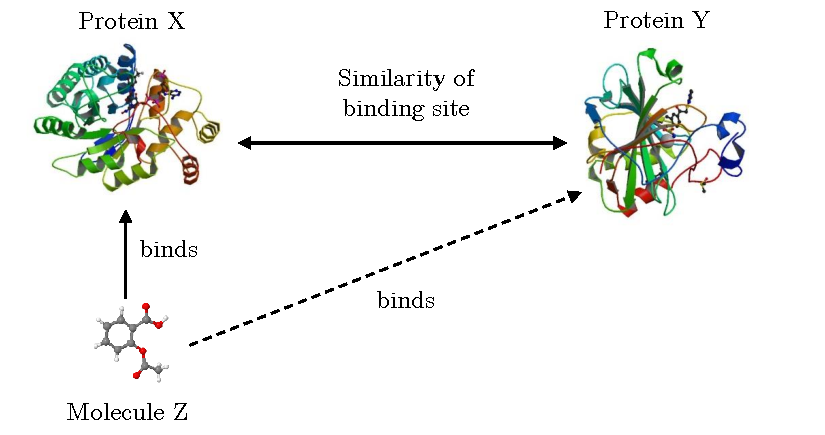
\includegraphics{fig1-7}
    \caption{Drug repositioning using protein structure and binding site. The 3D structure of proteins and their respective binding sites can be compared using a scoring function. On this basis, it is assumed that similar binding sites can bind the same ligand. For instance, knowing that protein X has a similar binding site to the one in protein Y, and that molecule Z binds to protein X, one can forward the hypothesis stating that molecule Z should bind to protein Y too. Illustration from the Protein Data Bank.}
    \label{fig1-7}
\end{figure}

\cite{zahler2007inverse} performed an inverse screening (docking one compound over multiple binding sites) to characterise the off-target binding landscape of kinase inhibitors. This class of drugs, largely used in cancer therapy, has a notorious “promiscuous” behaviour. The virtual screening revealed a new enzyme, PDK1, as an off-target of indirubin. Here again, the prediction was validated in vitro via a phenotypic cell proliferation assay demonstrating the validity of the approach and providing insights regarding kinase inhibitors’ side-effects.

Finally \cite{kinnings2009drug} addressed drug resistant tuberculosis using molecular docking methods. The bacteria behind the condition can indeed sometimes resist the first-line drugs, and in such cases, the eradication of the pathogen becomes difficult. The authors followed a workflow called “selective optimisation of side activities” (SOSA), a technique developed to progressively move away from the original indication and optimise a compound across protein families \citep{wermuth2006selective}. Briefly, the methodology is composed of the following steps: Binding site extraction from 3D structure of protein sequences, identification of similar binding sites across the proteome using a search algorithm, and finally manual docking analysis to make sure the physical interaction is possible. From this pipeline, the group predicted the approved drugs entacapone and tolcapone (prescribed for Parkinson’s disease) to be potent against the enoyl-acyl carrier protein reductase, an enzyme essential for the synthesis of fatty acid in Mycobacterium tuberculosis. The drugs were experimentally proven to be active in vitro, using commercially available tablets. Even more interestingly, the new mode of action introduced with these two compounds could bypass the drug resistance encountered in M. tuberculosis, and provide a valuable treatment for affected patients.

Despite the mentioned successes, molecular docking strategies for drug repositioning suffer from drawbacks. First, 3D structural data must be available. Databases such as the Protein Data Bank (PDB) contain numerous records, however they are still very far from covering the whole proteome \citep{haupt2011old}. Secondly, it can be challenging to automatically recognise a binding site, in particular when the protein structure was crystallized without the ligand. Finally, as all methodologies generate a large number of false positives, experimental and manual validations are the only solution to evaluate the predictions. Sometimes a single amino acid difference will totally change the pharmacology of the binding site \citep{kruger2012mapping}, a difficult problem to handle when the structures are analysed and aligned in an automated fashion.

In conclusion, protein-based approaches are arguably the closest methodology to the actual physical interaction between a drug and a protein target. Docking approaches provide a detailed low level picture of the biochemical complex, yet still suffer from challenges on the modelling side. The identification of off-target proteins does not necessarily always yield repositioning opportunities, and the results always have to be interpreted in a broader biological context.

\subsection{Phenotype and side-effect-based approaches}

The phenotype can be defined as the set of characteristics or traits attributed to an organism. Examples of phenotypes are the morphology, developmental, biochemical or physiological properties \citep{phenotypewiki}. This concept is widely used in biological sciences, to express the high level observations made when looking at a living organism. The phenotype is arguably the most primitive interaction between the biomedical scientist and its object of study: While travelling across the world, Darwin built the evidence for evolution from the phenotype of barnacles \citep{darwin2009origin}. Gregor Mendel first described inheritance based on the traits observed in pea plants \citep{mendel1866versuche}. None of these scientists had any idea about the actual molecular mechanism responsible for the observed patterns, yet their phenotypic observations were strong enough to forward valid conclusions. This exercise is still very commonly practiced in clinical settings. Every time a doctor diagnoses a patient, he or she primarily relies on a phenotypic characterisation of the signs and symptoms present in the patient. As mentioned earlier in this chapter (section \ref{sec:opp}), phenotypic-driven screenings are also routinely performed within drug discovery pipelines. It actually appears to be the best technique to bring new medicine to market, according to a recent study \citep{swinney2011were}. This successfulness can be attributed to the fact that a phenotypic observation is a more accurate representation of the underlying system; the physiological context is preserved, as opposed to target-based assays, therefore in vitro lead compounds have better chances to stay active when scaling to animal models and eventually clinical trials \citep{duran2012recycling}.

Back to drug repositioning concerns, side-effects can also be seen as phenotypes. The sildenafil story emphasises their importance: No matter how potent a drug is in animal model or in in vitro assays, its true pharmacology will only appear during the clinical trials. Accurately characterising these side-effects can help to reposition a drug or reveal new interaction partners, as highlighted by two studies, summarised here (see Figure \ref{fig1-8}).

\begin{figure}[ht]
    \centering
    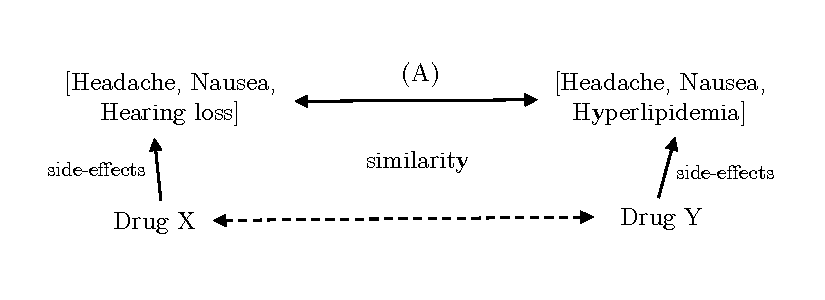
\includegraphics{fig1-8}
    \caption{Drug repositioning using phenotype information. Knowledge about the phenotypic outcome triggered by a drug can be used in order to establish relative similarities. (A) The diagram illustrates a theoretical example using reported side-effects: The more side-effects are commonly shared by two drugs, the more similar these two drugs are. The similarity can be used to either derive potential off-targets or new indications.}
    \label{fig1-8}
\end{figure}

Drugs with similar target binding profiles cause similar side-effects (\cite{fliri2005analysis} and \cite{fliri2007analysis}). Starting from this rationale, \citep{campillos2008drug} defined the side-effect profiles for approved drugs, then used similarity among these to identify the drug’s off-targets. The side-effects were first extracted using text-mining from package inserts \citep{campillos2008drug}, in order to build a statistical model informing about the likelihood for two drugs to have a common target. The authors then focused on compounds from different therapeutic categories, yet with a high probability of sharing a target according to the model. They experimentally tested 20 of such predictions, validating 13 of them, 11 with an inhibition constant under 10 micromolars. The originality of the method demonstrates the molecular relevance of side-effects, and their potential to identify off-targets and reassign a therapeutic molecule to a new indication. An interesting aspect of this approach is the representation of side-effects. Just as any phenotypic manifestation, words or terms, derived from observations, are still the best way to express them. For this study, the authors used the Unified Medical Language System (UMLS - \cite{bodenreider2004unified}), a controlled vocabulary provided by the National Health Institute. From the experimental validation shown by the research group, one can infer that ontologies and controlled vocabularies indeed have the potential to generate sound predictions.

Another approach was presented by \citep{yang2011systematic}. The authors used side-effects from the database SIDER to link diseases and extract drug repositioning opportunities. Chemicals were linked to pathologies using the information available in pharmacogenomics knowledge base (PharmGKB - \cite{whirl2012pharmacogenomics}). The approach leverages evidence showing that drugs used to treat similar diseases have similar side-effects. In this respect, side-effects can be indicators of a common underlying mode of action, and two drugs sharing a significant number of side-effects can be used to treat the same pathology. Sometimes a side-effect can also be deleterious in one case and beneficial in another. For instance hypotension is usually thought of as an unfavourable side-effect, yet the compounds producing such an effect could be used as antihypertensive agents. Following this hypothesis, a predictive model (Naive Bayes) was then built in order to assign drugs to diseases on the basis of side-effects. The high performance of the evaluation demonstrated the relevance of the methodology. The authors further developed a tool to predict new indications for compounds under development in a systematic fashion. No experimental validation was presented, yet a robust evaluation of the methodology was performed.

Fifty years ago, the phenotype was at the centre of drug discovery. With the advent of molecular biology, it was progressively replaced by the target-based paradigm \cite{duran2012recycling}. Phenotype-based approaches are still interesting for drug discovery, as they report the effect of a given substance on the level of whole organisms, which may be more representative for clinical applications. Thanks to the recent development of ontologies and methods (\cite{hoehndorf2011phenomenet} and \cite{hoehndorf2007representing}), it seems that the biomedical community has now better way to record, capture and align phenotypic information.

\subsection{Genetic variation-based approaches}

Closer to the molecular level, genetic variations can also provide valuable insights regarding drug repositioning opportunities. Due to the recent implementation of high-throughput DNA sequencing methods and analysis pipelines, it indeed becomes increasingly cheaper to sequence individuals and study their genotypes. From the information generated, one can isolate common mutations in the DNA that are significantly associated with a phenotypic trait. This method is known as genome-wide association study (GWAS) and is typically used to relate a single-nucleotide polymorphism (SNP) to a disease. The data about SNPs and their association to pathologies is indexed in databases, such as the one provided by National Human Genome Research Institute (http://www.genome.gov/gwastudies/). Using this resource, \citep{sanseau2012use} performed an analysis to unveil potential new indications for protein targets from GWAS. The logic behind the approach is that the association between a SNP and a trait from a GWAS can be extrapolated as a relation between a gene and a disease (if the only traits considered are diseases - see Figure \ref{fig1-9}). Then knowing that a drug targets the given gene product, one would expect for the indication of the drug to be the same as the trait studied in the GWAS. For instance, in the gene encoding 3-hydroxy-3-methylglutaryl-CoA (HMGCR), a SNP was significantly associated with the trait LDL cholesterol \citep{kathiresan2008six}. A class of drugs, the statins, are known to target this gene product and are indicated as cholesterol lowering agents (hypercholesterolemia). The authors identified 97 of such cases, where the SNPs support the current drug indication and give more confidence to the biological role of the protein. On the contrary, for 123 associations, the authors reported a mismatch between the trait associated with the gene and the current indication of the drug; these associations have been inferred as repositioning opportunities. For example, denosumab is a monoclonal antibody indicated for the treatment of osteoporosis and bone cancer. Its main target, the protein TNFSF11 (tumor necrosis factor superfamily, member 11) contains a SNP paired with Crohn’s disease \citep{franke2010genome}. Based on this evidence, denosumab could be tested for this later condition. Another example reported by the authors is nepicastat, a small molecule indicated for cocaine addiction and post-traumatic stress disorder. The target of the compound, DBH (dopamine beta-hydroxylase), has been associated with the trait smoking cessation in a GWAS \citep{furberg2010genome}. This result suggests a new and unreported use for nepicastat, as a drug for smokers willing to stop.

\begin{figure}[ht]
    \centering
    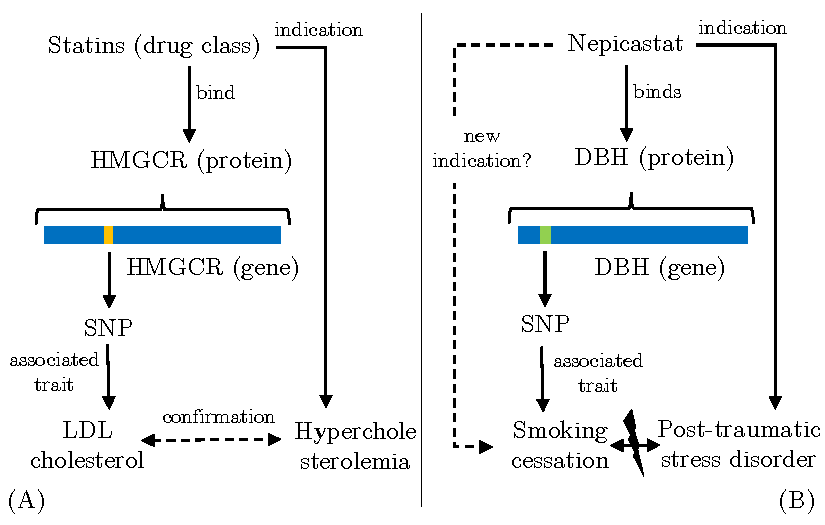
\includegraphics{fig1-9}
    \caption{Drug repositioning using genetic information. (A) Single-nucleotide polymorphism (SNP) are associated with a phenotypic trait, here LDL cholesterol. The gene where the SNP is found (HMGCR) encodes for a protein, targeted by statins (drug class). Statins are indicated as cholesterol lowering agents, which is confirmed by the trait associated with the SNP. (B) Sometimes the trait associated with the SNP diverges from the indication of the drug, as shown on the diagram (post-traumatic stress disorder against smoking cessation). In such cases, a repositioning hypothesis can be generated. Examples are detailed in the text. See \cite{sanseau2012use} for more explanations.}
    \label{fig1-9}
\end{figure}

The methodology presents some pitfalls, as shown by the prediction made for NOS2 (nitric oxyde synthase 2) inhibitors to be active against psoriasis; clinical trials unfortunately failed to show any significant effects. The gene-disease relation is indeed complex in practice, and sometimes more information is needed to appreciate the potential effect of a drug. Moreover, since GWAS does not provide any information regarding the direction of the pharmacological effect and it is difficult to know for instance whether an agonist or antagonist should be used to produce an outcome. Despite these restrictions and because of the impressive recent progress made in genome sequencing, this approach, or a related methodology, might gain in importance in the coming years.

\subsection{Disease network-based approaches}

Traditionally, diseases have been grouped together, on the basis of the cause of the pathology (e.g. infection) or the biological dysfunction observed (e.g. uncontrolled cell growth) for instance. As similar diseases are treated in a similar fashion, a better characterisation of the relation holding between pathologies can generate drug repositioning hypotheses. I will briefly present some of the work done in this direction, on the construction of a “diseasome” or network of relationships between diseases (see Figure \ref{fig1-10} for summary).

\begin{figure}[ht]
    \centering
    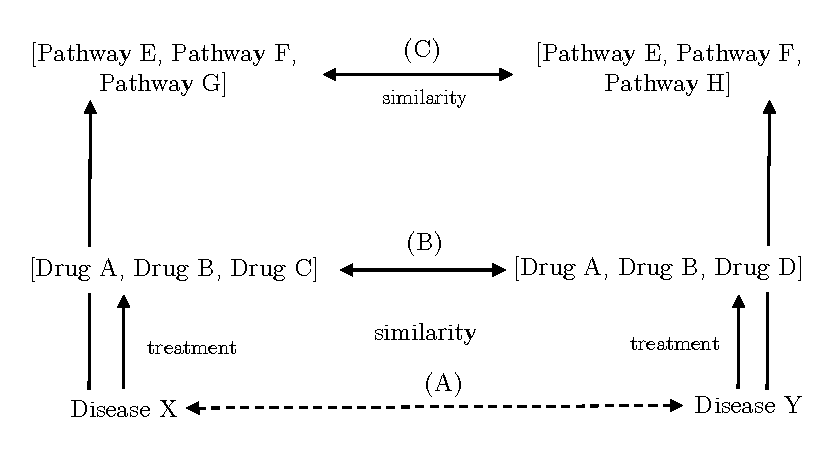
\includegraphics{fig1-10}
    \caption{Drug repositioning using disease relationships (diseasome). The similarity between two diseases (A) can be calculated by looking at the shared drugs used for the treatment of these diseases (B) or at the commonly shared pathways (C). When applied to all diseases, one can build a “diseasome” or disease map, useful to relate indications and find drug repositioning opportunities.}
    \label{fig1-10}
\end{figure}

\cite{chiang2009systematic} defined diseases from the list of drugs used in their therapies and off-label indications. Despite being fairly simplistic, the rationale is backed by successful examples and commonly practiced in clinical settings. The authors performed an associative indication transfer, namely, given two similar diseases, proposing to use a drug indicated only for one of them as a therapy for the other. From 700 diseases and 2000 drugs, over 150’000 new associations were generated. Interestingly, the new indications are in agreement with clinical trials data, the predicted new usage has often been reported by doctors (12 fold enrichment against random). For instance, atorvastatine, a cholesterol lowering agent, was predicted to be active for asthma, Crohn's disease and myocardial infarction; all these associations have been positively reported in clinical trials, proving confidence in the methodology. For the same drug, some of the new associations have no clinical evidences, such as activity in breast cancer and osteosarcoma. Accordingly, it is possible to investigate the action of the drug for these pathologies. This work illustrates one possible approach relating diseases; two other methodologies presented now respectively construct the network from shared pathways and functional modules.
The first one \citep{li2009pathway} built a map linking diseases from public resources (e.g. Reactome \citep{matthews2009reactome}, Kegg pathways \citep{goto1996organizing} and text-mining. Diseases with commonly dysregulated pathways were deemed to be similar. The properties of the resulting graph were analysed and the authors showed how their work can provide new insights about disease relationships. No analysis for repositioning opportunities were performed, yet the map can serve as a starting point to identify similar conditions, on which one can perform an indication transfer as before.
Finally, \cite{suthram2010network} constructed a disease graph from gene expression profiles and protein networks. An analysis revealed 59 functional modules, shared by half of the diseases studied. These modules relate pathologies on their molecular basis and help to better understand the internal wiring of the system. Similarly to other methods, once the disease network is created, drug repositioning hypotheses can be generated.
As a conclusion, despite not directly addressing drug repositioning, disease maps can provide valuable insight regarding the usage of a drug. Such approaches also question the current way of classifying diseases, by considering molecular information as signature or definition.

\subsection{Machine learning and concepts combination approaches}

The approaches presented before mostly focus on one of the concepts of the map shown on Figure \ref{fig1-4} and orient their analysis around it. It is also perfectly possible to use a combination of these biomedical descriptors to train a machine-learning algorithm and then generate predictions out of the statistical model (see Figure \ref{fig1-11}). Two recent studies address drug repositioning from this perspective. In both cases, first a series of biomedical heuristics is defined, then the model is trained on known data and predictions are made.

\begin{figure}[ht]
    \centering
    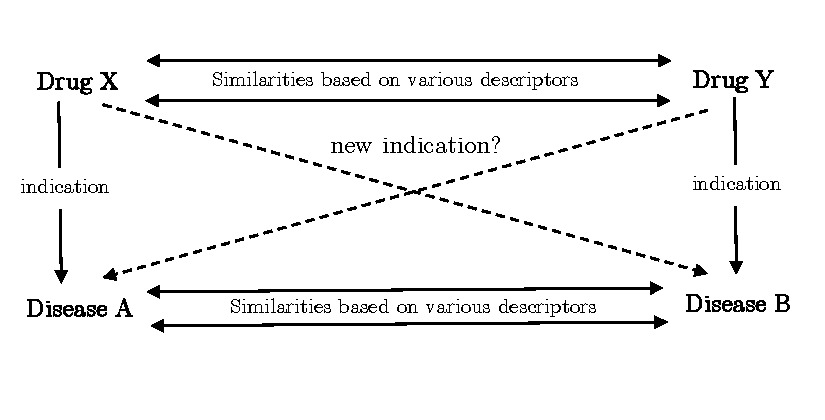
\includegraphics{fig1-11}
    \caption{Drug repositioning using a combination of descriptors. A machine learning algorithm is trained over a series of features, such as chemical similarity, shared target proteins, etc… After evaluation of the model, some repositioning predictions can be generated from the statistical learning.}
    \label{fig1-11}
\end{figure}

The first method presented is called PREDICT \citep{gottlieb2011predict}. In order to train the machine-learning algorithm, the authors decided to represent separately drug-drug and disease-disease associations. Drug-drug associations were characterised from fingerprinting of their chemical structure and the reported and predicted list of side-effects. These drug-drug associations were further enriched with information related to the targets of the drugs: the sequence similarity, distance in the protein-protein interaction network and semantic similarity of their GO annotations. The disease-disease associations were more simply characterised based on their semantic similarities calculated over the Human Phenotype Ontology (HPO) from the annotations present in the Online Mendelian Inheritance in Man (OMIM) database. From these gold-standard associations, the authors trained a logistic regression classifier to recognise real associations from fake ones. The model was evaluated against the predictions made by other methodologies, such as guilt-by-association and CMap approaches \citep{lamb2006connectivity}, presented earlier in this chapter. The evaluation shows little overlap between the various methodologies; it is difficult to align the various datasets, as often the diseases and drugs considered are different. Some drug repositioning predictions were then generated and evaluated from clinical trials data. Around a third of the predictions were reported as already investigated, giving confidence in the outcome of the methodology. In the last part of their work, the authors substituted the disease-disease associations based on phenotypic similarity with gene expression profiles. The idea behind this step was to test the developed method for personalised medicine: Assuming one has access to the gene expression profile of a patient, can PREDICT find the best drug to administer to the individual? Results were encouraging; the method reports high recall and specificity (area under curve of 0.92 obtained from receiver-emitter curve), providing a tangible proof-of-concept for the algorithm.

The second method presented \citep{napolitano2013drug} is very similar to PREDICT. The main difference comes from the machine-learning methodology, which was Support Vector Machine (SVM) in this study. The algorithm was used to predict therapeutic categories of the Anatomical Therapeutic Chemical Classification System (ATC), misclassifications being re-interpreted as drug repositioning hypotheses. The researchers also incorporated structural similarity, protein-protein interaction network distance and gene expression data as starting features to train the SVM. After standard machine-learning evaluation procedures, the authors derived repositioning predictions. The main hypotheses were anthelmintics compounds to be active as antineoplastic agents and antineoplastic drugs to be used as systemic antibacterials.

Machine-learning based approaches to drug repositioning provide a way to combine various descriptors into one statistical model, with the aim of increasing the accuracy of the predictions. The techniques presented however face some important pitfalls. One of them is the interpretation of the repurposing hypotheses: the statistical model is a black box, hiding the rational evidences of why a compound was chosen. Most of the hypotheses end up being obvious cases, easily explainable for a biologist by looking at the chemical structure or known off-targets of the compounds. This result is maybe due to an over-training of the machine. Finally, one can question the biomedical meaningfulness of integrating a large number of descriptors; since diseases are subtle and unique, too much information risks blurring the outcome by overlooking important biological mechanistic details.

\subsection{Summary}

A variety of approaches have been tried in order to computationally repurpose drugs. The field is still in its infancy, as revealed by two factors.

First, it is still not clear which method provides the best results and why. The only absolute way to evaluate the predictions is when a drug will be routinely indicated in the clinic from a hypothesis generated in silico; as far as I know, there is no compelling story illustrating this yet. It is not surprising; developing a new drug is a long process, taking over twelve years to achieve and trapped with legal and economic hurdles. Knowing that the first study reported by PubMed for the keyword search “computational drug repositioning” dates to 2006 \citep{an2006large} (or 7 years before the time of writing), it seems realistic not to find any clinical examples yet.

Secondly, each method addresses the drug repositioning problem from a different angle or biomedical concept, which complicates the evaluation process. Objectively integrating the results from the various approaches is a difficult task, as the starting datasets are about different molecules and diseases and produce different type of outcomes. It would be beneficial for the community to have a standard dataset, covering the legal indications, as well as the known and confirmed alternative ones. Computational methods could use such a resource to benchmark their performance and evaluate their predictive power and perform error analysis.
Immaturity also means creativity in this case, illustrated by the numerous methods implemented. Table \ref{table1} and \ref{table2} provide a summary of the approaches presented, alongside their respective strengths and weaknesses.

\afterpage{%
    \clearpage% Flush earlier floats (otherwise order might not be correct)
    \thispagestyle{empty}% empty page style (?)
    \begin{landscape}% Landscape page
            \scriptsize
        \centering % Center table
        \begin{tabular}{ | p{2cm} | p{3cm} | p{4cm} | p{3cm} | p{4cm} | p{2cm} | p{3cm} | }
    \hline
    Biomedical concept & Rationale & Biomedical advantages & Technical advantages & Biomedical pitfalls & Technical pitfalls & References \\ \hline
    Chemical structure & Similar chemical structures have similar biological outcomes (similar property principle) & Off-target identification - Straigtforward interpretation - Can be used on new chemical structures with unknown activities & Fast algorythm available to encode and search for chemical structures (fingerprint) - Large number of structures available & Prediction can have weak binding, not nessecary pharmacologically active - Small changes made to a molecular structure can change a lot the biological outcome - Compounds may undergo chemical modifications by the cell (pro-drugs), therefore original structure is not so helpful & Chemical structures information in databases is sometimes erronous & 16986201 - 19881490 \\ \hline
    Gene expression (mRNA) & A biological state can be defined by the list of genes under or over-expressed (signature) in the given state. It is possible to define disease states and drug states (Connectivity Map) and analyse their relative similarities. & Systematic characterisation of the biological function - No previous knowledge required about diseases or protein targets & Assay well understood and cheap - Connectivity Map data freely available and extending & Too simplistic to characterise some states, important mechanistic aspect can be overlooked & Selection of the representative genes is challenging - Connectivity Map data were recorded on cancer cell, might not feat all types of diseases or it can bias the signature & f. ioro - 21849665- 21849664- 17010674 - 21641545 - cmap paper\\ \hline
    Protein & Computational modelling of the physical binding of a drug to a protein & Off-target identification - Straigtforward interpretation - Can be used with chemical structures with unknown activities - Close to biochemical reality & Numerous tools available to perform docking studies & Predicting a binding is challenging because of molecular dynamics - High number of false positive predictions& Structural databases are not complete, not all proteins are considered & \cite{ashburner2000gene} - 21441562 - 20808948 - 18022559‎ - 19578428\\ \hline
        \end{tabular}
        \captionof{table}{Summary of drug repositioning approaches.}% Add 'table' caption
        \label{table1}
    \end{landscape}
    \clearpage% Flush page
}

\afterpage{%
    \clearpage% Flush earlier floats (otherwise order might not be correct)
    \thispagestyle{empty}% empty page style (?)
    \begin{landscape}% Landscape page
            \scriptsize
        \centering % Center table
        \begin{tabular}{ | p{2cm} | p{3cm} | p{4cm} | p{3cm} | p{4cm} | p{3cm} | p{2cm} | }
    \hline
    Biomedical concept & Rationale & Biomedical advantages & Technical advantages & Biomedical pitfalls & Technical pitfalls & References \\ \hline
    Genetic & Genomic identification of phenotypic traits & Potentially closer to individual patients (SNP) & Large amount of SNP information already available and growing everyday - Decreasing cost of sequencing& Does not provide mechanistic details nor context & Genome data analysis is still challenging & 22491277\\ \hline
    Disease & Similar diseases receive similar treatment & Systemic characterisation and classification & Various methodologies can build the diseases map & Does not directly address drug repositioning & Highly rely on curated knowledge & 19571805 - 19194489 - 20140234\\ \hline
    Combination & Training of a machine-learning algorithm from a series of descriptors & Incorporation of multiple dimensions, providing a more consistent representation of the biological phenomenon & Numerous machine-learning program and methodologies available & Biological interpretation dificult (black box approach) - Risk of over training the system - Does not provide mechanistic details & Choice of the heuristics is challenging & 21654673 - 23800010\\ \hline
    Biological process and molecular function & Formal representation of the mode and mecanism of action & Systemic characterisation of the biological role - Mechanistic description & Large amount of information available - Data integration & Predictions can have weak binding, not nessecary pharmacologically active & Highly rely on curated knowledge & N.A.\\ \hline
        \end{tabular}
        \captionof{table}{Summary of drug repositioning approaches (continued).}% Add 'table' caption
        \label{table2}
    \end{landscape}
    \clearpage% Flush page
}

To conclude, computational drug repositioning appears as a topic of growing interest in the scientific community, as inferred from Figure \ref{fig1-13}. A series of methods have been developed in the last 5 years, summarised and discussed in this chapter. Drug repositioning is a subset of a larger problem type: Indication discovery and network biology \citep{hopkins2008network}. In can be summarised as taking advantage of our increasing knowledge about systemic behaviour to computationally design smart drugs.
The conclusions drawn from this state-of-the-art review oriented my work and motivated me to explore drug repositioning from the perspective of biological processes and molecular functions.

\begin{figure}[ht]
    \centering
    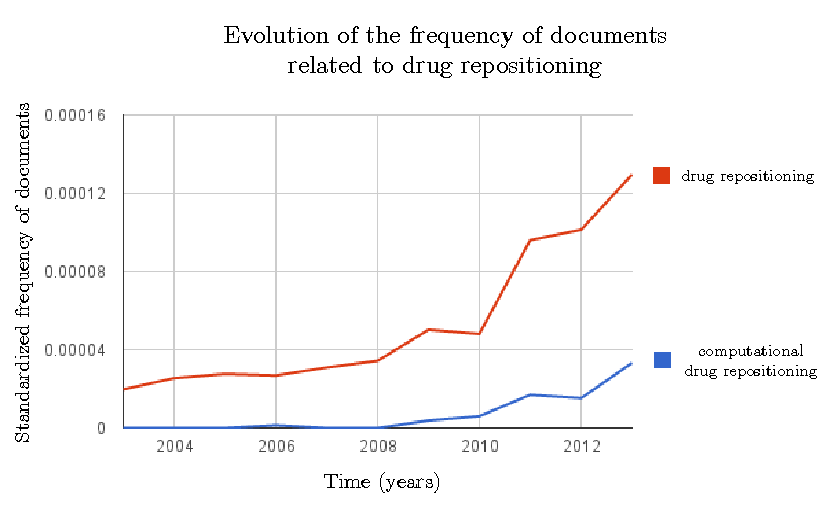
\includegraphics{fig1-13}
    \caption{Evolution trend of the documents related to drug repositioning. Standardised frequency: Number of documents indexed on PubMed for a search divided by the total number of articles published the same year. The higher, the more popular a topic is. The  frequency increases with the time for both searches, showing a growing interest in the domain.}
    \label{fig1-13}
\end{figure}


\section{Thesis: Biological process and molecular function for drug repositioning}

The previous section (\ref{approaches}) gave an overview of the various computational techniques developed for drug repositioning within the last decade. I believe that the most promising results appear to come from gene expression analyses (section \ref{expression}), driven by the large amount of public data available and encouraging in vivo results. Additionally, gene expression provides a functional insight about a biological state, valuable in practice: From a drug indication perspective, it is indeed much more pertinent to know what a molecule does (role or function) rather than what it physically looks like (structure).

Following this philosophy, I argue in favour of the mode of action, as a means to formally define the function of a drug. The concept brings unique assets, such as bridging from the molecular to the phenotype level, as well as providing a discrete mechanistic understanding of the role of a drug.

In this section, I will introduce my thesis, namely the vision and the rationale behind the approach of using curated knowledge of biological processes and molecular functions to characterise the drug repositioning landscape. Processes and functions provide a flexible abstraction layer in between biochemistry and systems biology. My thesis work is based on a computational characterisation of the mode of action of marketed drugs. This notion is particularly relevant to drug repositioning, as the concept provides mechanistic insights regarding the broad pharmacological action of a drug. Moreover, a compound can also have several modes of action, representing the various biological processes the molecule can perturb from its polypharmacology.

\subsection{Rationale}

Knowing the potential role a drug can play in a living organism such as a human body enables one to logically re-use the compound for a different indication. Moreover, a drug binds to multiple proteins, themselves involved into multiple biological processes (see section \ref{sec:opp}). Therefore a drug can potentially play a multitude of roles, or in other words can have several MoAs, which are accountable for its polypharmacology.

In practice, the biological roles of drugs are described as mechanism or mode of actions. The mechanism of action can be defined as the biochemical interaction that gives rise to the pharmacological effect of a drug. For instance, the term “phosphodiesterase-5 binding” is the mechanism through which the sildenafil molecule produces its action. Similarly, the mode of action (MoA) defines in a more abstract fashion the broad activity of the molecule on an organism. The terms “pro-penile erection agent” and “vasodilator” both are valid modes of action (MoA) of the same sildenafil molecule. Another example of MoA is “anti-blood coagulant”, representing the capacity of a drug to inhibit or decrease the extent of blood coagulation (see Figure \ref{fig1-12} for example).

\begin{figure}[ht]
    \centering
    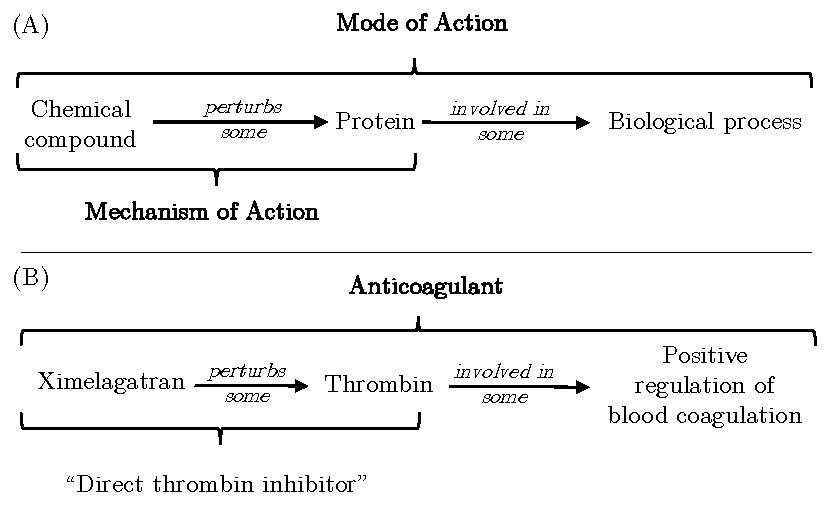
\includegraphics{fig1-12}
    \caption{Schematic representation of the concept of mechanism and mode of action. (A) The mechanism of action can be defined as the physical activity of the ligand on a protein target. The mode of action characterises the pharmacology of the small molecule in the context of the organism. (B) Examples related to blood coagulation illustrating the usage of the mechanism and mode of action concepts.}
    \label{fig1-12}
\end{figure}

The concepts of mode and mechanism of action are broadly used in drug discovery; they help to classify drugs into therapeutic groups. Even more importantly, a chemical is assigned as a treatment to a disease because it exhibits a particular MoA. One example is the case of high blood pressure, a common medical condition leading to an increased risk of heart attacks and strokes \citep{hypertensionnhs}. In order to chemically decrease the blood pressure, several biological solutions can be considered. A first approach could remove the excess of salt from the body, thereby decreasing the tension in the blood vessels (//cite something). An alternative solution could inhibit the vasoconstrictive signalling of a hormone (//cite something). Finally, it is also possible to act directly on the cells physically narrowing the vessels and preventing their unwanted action this way (//cite something). Now if a chemical was known to be capable of producing any of these biological actions, it would then be possible to indicate it for the treatment of the hypertension. This logic puts emphasis on the mechanistic details of the pharmacological effect. The MoA explicitly characterises the function of the drug in the cellular machinery, and helps to appreciate its overall effect. As opposed to statistical methods and black box techniques, the explicit reasons why a particular drug shows a particular outcome can be derived from curated knowledge in a systematic fashion.

A MoA-based approach comes with unique theoretical advantages. First, it provides a systematic high-resolution picture of the function of drugs, just like gene expression experiments. Moreover, this characterisation of the function is discrete and granular. Unlike gene expression data (CMap), the function of the molecule is not vaguely summarised in a gene expression signature. MoAs are discrete categories, and a compound can be put in many of them, as illustrated with hypertension. In this respect, the MoA can be seen as the equivalent of a protein’s functional annotations \citep{ashburner2000gene}, but for drugs. Finally, the MoA provides a unique level of abstraction over biological systems: It logically links the biochemical mechanistic interaction, as studied with docking and chemical similarity, to a high level phenotypic process, such as a disease or a side-effect.

\subsection{Towards the specification, implementation and analysis}

The computational use of the MoA to repurpose drugs comes with obstacles. I gave in the previous section some informal examples of MoAs: vasodilator, anti-blood coagulant, anti-ageing agent, etc. However, in order to provide helpful information, all MoAs (or a large number at least) have first to be unambiguously and formally defined. From these examples and Figure \ref{fig1-12}, the reader can see that MoAs are terms, boxes or categories; classical mathematical frameworks used in biology and bioinformatics, such as statistics, do not provide any means to address this concern.

A MoA describes logical events happening inside the complex cellular machinery: Intuitively, an anti-blood coagulation agent is a type of compound capable of modifying the activity of a protein target somehow involved in the blood coagulation. Therefore representing the axioms or logical links underlying these statements can set the basis to derive new MoA categories, as shown in Figure \ref{fig1-12}. However, the definition of MoAs from this perspective will necessarily rely on existing knowledge or data. From the example before, it is indeed necessary yet sufficient to know first that a drug binds a particular protein and secondly that this protein is involved in the coagulation process in order to formally derive the MoA of the compound.

The implementation of the rationale is described in the rest of this document and organised as follow.

\subsubsection{Chapter 2 - Description logics and biomedical knowledge (Specification)}

Before representing modes of action and using them to classify drugs, the specifications of the system have first to be clearly determined. How are the logical connections between biological processes and molecules going to be represented? Will the system scale and work even with large biomedical input size? What is meant by biological knowledge? How does it fit currently available biomedical data? These questions will be addressed in Chapter 2, introducing description logics as a mathematical framework of choice to perform the MoA implementation later on. I propose an analogy considering living organisms as machines to describe a portion of the biomedical knowledge, relevant to drug discovery.

\subsubsection{Chapter 3 - The Functional Therapeutic Chemical Classification System (Implementation)}

The specification finds an implementation in Chapter 3, with the Functional Therapeutic Chemical Classification System (FTC). The classification features a representation of over 20’000 modes and mechanisms of action categories, inside which approved drugs have been classified. The work done was evaluated against existing solutions and is publicly available via a web application. As expected, on average drugs are present in numerous MoA categories. This observation can be used to perform different types of analysis and generate drug repositioning hypotheses.

\subsubsection{Chapter 4 - Systematic drug repositioning analysis}

The content of the FTC is analysed in Chapter 4 from different perspectives. First, the relationship between the concepts of a drug’s structure, function and indication is discussed in this chapter. Secondly a list of drug repositioning hypotheses is derived from this preliminary characterisation, covering a wide range of therapeutic areas. The hypotheses are used to analyse in a systematic fashion the drugs’ off-label uses. Finally hypertension and Alzheimer's disease have been selected as use-cases in order to further investigate drug repositioning opportunities.

\subsubsection{Chapter 5 - Outlook}

The outcomes of the thesis work are put into perspective: What part of the drug discovery process has been covered? What are the next logical steps for future work? Can the mode of action representation be further improved and how? The pitfalls encountered during the work are discussed and I present my vision towards a simpler knowledge representation system for the biomedical domain. Chapter 5 also discusses alternative analyses that can be performed with the content of the FTC, in particular against gene expression data.
